\chapter{Linear Analysis of the Numerical Methods}
\label{chp:AnalNumMethod}
An important property of a numerical method is convergence. Convergence guarantees that as the spatial and temporal resolution of a numerical method is increased, then the numerical solution approaches the solution of the partial differential equations they approximate. 

For linear partial differential equations the Lax-equivalence theorem states that a numerical method is convergent if and only if it is stable and consistent \cite{Lax-Richtmyer-1956-267}. A numerical scheme is consistent if the error introduced by the numerical method over a time step approaches zero as the spatial and temporal resolution is increased. While a numerical method is stable if the errors from previous time steps are not amplified in subsequent time steps.

Another important attribute of a numerical method modelling dispersive wave equations, such as the Serre equations is its dispersion properties. The dispersion relation of a system determines the phase and group velocity of travelling waves in that system. The Serre equations possess a dispersion relation that well approximates the dispersion relation given by linear theory for water waves \cite{Barthelemy-2004-315}. Therefore, how well the dispersion relation of a numerical method approximates the dispersion relation of the Serre equations is of particular interest.

We analysed the convergence and the dispersion properties of our numerical methods for the linearised Serre equations with a horizontal bed. The effect of variations in the bed and nonlinear terms are important when studying the convergence properties of our methods for solving the full Serre equations. However, these effects greatly increase the complexity of the convergence analysis. We therefore, restrict ourselves to the study of the linearised Serre with a horizontal bed to offer some insight into the convergence properties of our numerical methods without having to deal with this additional complexity. In general, we would expect that a numerical method that has poor convergence properties for the linearised Serre equations with a horizontal bed will also have poor convergence properties when the bed and nonlinear terms are included. The dispersion properties are derived from the linearised Serre equations with variable bathymetry having no effect \cite{Zoppou-etal-2017}, therefore the presented analysis of the dispersion properties of the numerical methods is a complete analysis.


The linear analyses of convergence and dispersion properties rely on establishing a relationship of the form

\begin{equation}
\label{eqn:linearanalaim}
\begin{bmatrix}
h \\G
\end{bmatrix}^{n+1}_j = \matr{E} \begin{bmatrix}
h \\G
\end{bmatrix}^{n}_j
\end{equation}
 where $\matr{E}$ is the evolution matrix relating the conserved quantities $h$ and $G$ at time level $t^n$ with the conserved quantities at time level $t^{n+1}$, which is independent of $n$ and $j$. The evolution matrix $\matr{E}$ is obtained in the analyses by propagating Fourier modes through the numerical scheme. By analysing the properties of $\matr{E}$ we can determine the convergence and dispersion properties of its associated numerical method.
 
 We derive $\matr{E}$ in \eqref{eqn:linearanalaim} for the second-order FEVM and perform the convergence and dispersion analysis. We will then present the results of these analyses for all the other numerical methods in this thesis.
 
\section{Linearised Serre Equations with a Horizontal Bed}
The Serre equations with a horizontal bed \eqref{eqn:FullSerreNonConHorizbed} are linearised by considering waves as small perturbations $\delta\eta$ and $\delta\upsilon$ on a flow with a mean height $H$ and a mean velocity $U$ respectively. So we have
\begin{subequations}
	\label{eq:pertubation}
\begin{align}
h(x,t) &= H + \delta \eta(x,t) + \mathcal{O}\left(\delta^2 \right), \\
u(x,t) &= U + \delta \upsilon(x,t) + \mathcal{O}\left(\delta^2 \right),
\end{align}
\end{subequations}
where $\delta \ll 1$. These waves are relatively small so terms of order $\delta^2$ are negligible. We substitute \eqref{eq:pertubation} into the Serre equations and neglect terms of order $\delta^2$ to obtain

\begin{subequations}
	\begin{align}
		\label{eqn:LinCont}
		&\frac{\partial  \left(\delta\eta \right)}{\partial  t} + H\frac{\partial  \left(\delta\upsilon \right)}{\partial  x} + U\frac{\partial  \left(\delta\eta \right)}{\partial  x}  = 0, \\
	\label{eqn:LineMome}
	&H\frac{\partial  \left(\delta\upsilon \right)}{\partial  t} + gH\frac{\partial  \left(\delta\eta \right)}{\partial  x} + UH\frac{\partial  \left(\delta\upsilon \right)}{\partial  x} - \frac{H^3}{3}\left(U\frac{\partial^3  \left(\delta\upsilon \right)}{\partial  x^3} + \frac{\partial^3  \left(\delta\upsilon \right)}{\partial  x^2 \partial  t}  \right)  = 0
	\end{align}	
and for $G$
\begin{equation}
	G = UH + U \delta \eta + H \delta \upsilon -\frac{H^3}{3} \frac{\partial^2 \left(\delta\upsilon \right)}{\partial x^2}.
	\label{eqn:LinConSerreGu0}
\end{equation}	
	\label{eqn:LinConSerre}
\end{subequations}
These equations can be reformulated into conservation law form for the quantities $\eta$ and $G$
\begin{subequations}
	\begin{align}
	\label{eqn:LinContG}
	&\frac{\partial  \eta}{\partial  t} +\frac{\partial}{\partial  x} \left(H\upsilon + U \eta\right) = 0, \\
	\label{eqn:LineMomeG}
	&\frac{\partial  G}{\partial  t} + \frac{\partial}{\partial  x}\left(UG + UH\upsilon + gH \eta\right) = 0
	\end{align}
	where
	\begin{equation}
	G = UH + U \eta + H \upsilon -\frac{H^3}{3} \frac{\partial^2 \upsilon }{\partial x^2}.
	\label{eqn:LinConSerreG}
	\end{equation}
	\label{eqn:LinSerreG}	
\end{subequations}
We have absorbed the $\delta$ factor into the corresponding $\eta$ and $\upsilon$ terms to simplify the notation.

\section{Evolution Matrix}
To derive the evolution matrix, $\matr{E}$ we study the behaviour of \eqref{eqn:LinSerreG} when $\eta$ and $\upsilon$ are Fourier modes. For a general quantity $q$ a Fourier mode is
\begin{equation}
q(x,t) = q(0,0) e^{i\left(\omega t + kx\right)}
\label{eqn:FourierNode}
\end{equation}
where $k$ is the wavenumber , $\omega$ is the frequency and $i$ is the imaginary number. A consequence of a quantity $q$ being a Fourier mode represented on a uniform temporal and spatial grid is that for any real numbers $m$ and $l$ we have
\begin{equation}
q^{n + m}_{j + l} = q^n_j e^{ i \left(m \omega \Delta t + l k \Delta x\right)}.
\label{eqn:fourierfactor}
\end{equation}
Because $\eta$ and $\upsilon$ are Fourier modes then so is $G$. Furthermore, the cell averages of these quantities $\overline{\eta}$, $\overline{\upsilon}$ and $\overline{G}$ are Fourier modes as well.

When all the quantities are Fourier modes the operators $\mathcal{R}^+_{j-1/2}$, $\mathcal{R}_{j}$, $\mathcal{R}^-_{j+1/2}$, $\mathcal{G}$, $\mathcal{F}_{j-1/2}$ and $\mathcal{F}_{j+1/2}$ from Chapter \ref{chp:HFVMMethod} only vary with $H$, $U$, $k$, $\omega$, $\Delta x$ and $\Delta t$ and hence are independent of $j$ and $n$. By combining these operators the evolution matrix $\matr{E}$ can be derived for the second-order FEVM for the linearised Serre equations with horizontal bed. Since all of the constituent operators are independent of $j$ and $n$ then $\matr{E}$ will also be independent of $j$ and $n$, as desired. We will now derive expressions for all these operators, following the structure laid out in Section \ref{sec:StructOverview}. Since the linearised Serre equations with a horizontal bed has no Source Terms, step (iv) will be skipped.   

\setcounter{subsection}{0}
\renewcommand{\thesubsection}{(\roman{subsection})} 
\subsection{Reconstruction}
Given $\overline{\vecn{\eta}}$ and $\overline{\vecn{G}}$ at $t^n$ the first step of our numerical method is to reconstruct $\eta$ and $G$ inside the $j^{th}$ cell at $x_{j-1/2}$, $x_j$ and $x_{j+1/2}$ using $\mathcal{R}^+_{j-1/2}$, $\mathcal{R}_{j}$ and $\mathcal{R}^-_{j+1/2}$ from \eqref{eqn:ReconforhwG}. Since, $\eta$ and $G$ are Fourier modes and therefore smooth we do not require non-linear limiters to ensure our scheme is TVD and so we use the slope $d_j = \left({-\bar{q}_{j-1} +\bar{q}_{j+1}}\right)/ \left({2\Delta x} \right)$ in the reconstruction. Applying \eqref{eqn:fourierfactor} to the reconstructions \eqref{eqn:ReconforhwG} with the centred slope approximation we obtain 

\begin{subequations}
	\label{eqn:RpmfactorFDVM}
	\begin{align}
	q^+_{j-\frac{1}{2}} &= \overline{q}_j - \frac{- \overline{q}_{j} e^{-ik\Delta x} + \overline{q}_{j} e^{ik\Delta x}}{4} = \left(1  - \frac{i\sin\left(k\Delta x\right)}{2} \right)\overline{q}_{j} = \mathcal{R}^+_{j-1/2}\overline{q}_{j} \\
	q_j &= \bar{q}_j = \mathcal{R}_{j} \bar{q}_j,\\
	q^-_{j+\frac{1}{2}} &=\overline{q}_j + \frac{- \overline{q}_{j} e^{-ik\Delta x} + \overline{q}_{j} e^{ik\Delta x}}{4} = \left(1  + \frac{i\sin\left(k\Delta x\right)}{2} \right)\overline{q}_{j} =\mathcal{R}^-_{j+1/2} \overline{q}_{j}.
	\end{align}
\end{subequations}   



\subsection{Fluid Velocity}
To calculate $\upsilon_{j+1/2}$ we use a second-order FEM. We begin our FEM for \eqref{eqn:LinConSerreG} with its weak formulation, obtained by multiplying \eqref{eqn:LinConSerreG} by a test function $\tau$ and integrating over the spatial domain $\Omega$
\begin{equation*}
\int_{\Omega}G \tau \; dx = UH\int_{\Omega} \tau \; dx + U \int_{\Omega} \eta \tau \; dx +   H\int_{\Omega} \upsilon \tau \; dx  + \frac{H^3}{3} \int_{\Omega} \frac{\partial \upsilon}{\partial x } \frac{\partial \tau}{\partial x }\; dx.
\end{equation*}
For $G$ we use the basis functions $\psi^+_{j - 1/2}$ and $\psi^-_{j + 1/2}$ defined in Appendix \ref{app:FEMIntegrals}, which means our approximation to $G$ is linear inside a cell with discontinuous jumps at the cell edges. For $\tau$ and $\upsilon$ we use the basis functions $\phi_{j-1/2}$, $\phi_{j}$ and $\phi_{j+1/2}$ defined in Appendix \ref{app:FEMIntegrals} so that $\tau$ and our approximation to $\upsilon$ are quadratic polynomials inside a cell and are continuous across the cell edges. Substituting the finite element approximations to these quantities and only integrating over the $j^{th}$ cell, we get
%define the basis functions in appendix

\begin{multline*}
\sum_j \int_{x_{j-1/2}}^{x_{j + 1/2}} \left(G^+_{j-1/2}\psi^+_{j - 1/2} + G^-_{j+1/2}\psi^-_{j + 1/2}\right) \begin{bmatrix}
\phi_{j-1/2}\\\phi_j \\\phi_{j+1/2}
\end{bmatrix}  \; dx =  \\ \sum_j UH\int_{x_{j-1/2}}^{x_{j + 1/2}}  \begin{bmatrix}
\phi_{j-1/2}\\\phi_j \\\phi_{j+1/2}
\end{bmatrix}  \; dx + \sum_j U\int_{x_{j-1/2}}^{x_{j + 1/2}} \left(\eta^+_{j-1/2}\psi^+_{j - 1/2} + \eta^-_{j+1/2}\psi^-_{j + 1/2}\right) \begin{bmatrix}
\phi_{j-1/2}\\\phi_j \\\phi_{j+1/2}
\end{bmatrix}  \; dx \\   +\sum_j H\int_{x_{j-1/2}}^{x_{j + 1/2}} \left(\upsilon_{j-1/2}\phi_{j - 1/2} + \upsilon_{j}\phi_{j}+ \upsilon_{j+1/2}\phi_{j + 1/2}\right) \begin{bmatrix}
\phi_{j-1/2}\\\phi_j \\\phi_{j+1/2}
\end{bmatrix}  \; dx \\ + 
\sum_j \frac{H^3}{3}\int_{x_{j-1/2}}^{x_{j + 1/2}} \left(\upsilon_{j-1/2} \frac{\partial \phi_{j - 1/2} }{\partial x} + \upsilon_{j}\frac{\partial \phi_{j} }{\partial x}+ \upsilon_{j+1/2}\frac{\partial \phi_{j + 1/2} }{\partial x}\right) \begin{bmatrix}
\dfrac{\partial \phi_{j - 1/2} }{\partial x}\\ \\\dfrac{\partial \phi_{j} }{\partial x}\\ \\\dfrac{\partial \phi_{j + 1/2} }{\partial x}   \end{bmatrix} \; dx.
\end{multline*}
Calculating all the integrals of the appropriate basis function combinations we get 
\begin{multline*}
\sum_j \frac{\Delta x}{6}\begin{bmatrix} G^+_{j -1/2} \\2 G^+_{j -1/2}+2 G^-_{j +1/2} \\ G^-_{j +1/2} \end{bmatrix} = \sum_jUH \frac{\Delta x}{6}\begin{bmatrix} 1 \\4 \\ 1 \end{bmatrix} +  \sum_j \frac{\Delta x}{6}U\begin{bmatrix} \eta^+_{j -1/2} \\2 \eta^+_{j -1/2}+2 \eta^-_{j +1/2} \\ \eta^-_{j +1/2} \end{bmatrix}\\ + \sum_j \left(H\frac{\Delta x}{30}\begin{bmatrix} 4 &2 &-1 \\2 &16 &2  \\-1 &2 &4 \end{bmatrix} + \frac{H^3 }{9\Delta x}\begin{bmatrix} 7 &-8 &1  \\-8 &16 &-8  \\1 &-8 &7  \end{bmatrix} \right) \begin{bmatrix} \upsilon_{j -1/2} \\\upsilon_{j} \\ \upsilon_{j +1/2} \end{bmatrix}.
\end{multline*} 
%minmod limiter for G
Using \eqref{eqn:RpmfactorFDVM}, we obtain

\begin{multline*}
\sum_j \frac{\Delta x}{6} \begin{bmatrix} \mathcal{R}^+_{j -1/2} \overline{G}_{j} \\2 \mathcal{R}^+_{j -1/2} \overline{G}_{j} +2 \mathcal{R}^-_{j +1/2} \overline{G}_{j}\\ \mathcal{R}^-_{j +1/2} \overline{G}_{j} \end{bmatrix} =   \sum_jUH \frac{\Delta x}{6}\begin{bmatrix} 1 \\4 \\ 1 \end{bmatrix} \\+  \sum_j \frac{\Delta x}{6} U \begin{bmatrix} \mathcal{R}^+_{j -1/2} \overline{\eta}_{j} \\2 \mathcal{R}^+_{j -1/2} \overline{\eta}_{j} +2 \mathcal{R}^-_{j +1/2} \overline{\eta}_{j}\\ \mathcal{R}^-_{j +1/2} \overline{\eta}_{j} \end{bmatrix}  \\\sum_j \left(H\frac{\Delta x}{30}\begin{bmatrix} 4 &2 &-1 \\2 &16 &2  \\-1 &2 &4 \end{bmatrix} + \frac{H^3 }{9\Delta x}\begin{bmatrix} 7 &-8 &1  \\-8 &16 &-8  \\1 &-8 &7  \end{bmatrix} \right) \begin{bmatrix} e^{-ik\frac{\Delta x}{2}}\upsilon_{j} \\\upsilon_{j} \\ e^{ik\frac{\Delta x}{2}}\upsilon_{j} \end{bmatrix} .
\end{multline*}
After simplifying
\begin{multline*}
\sum_j \frac{\Delta x}{6}\begin{bmatrix} \mathcal{R}^+_{j -1/2} \\2 \mathcal{R}^+_{j -1/2} +2 \mathcal{R}^-_{j +1/2}\\ \mathcal{R}^-_{j +1/2} \end{bmatrix} \overline{G}_{j} = \sum_jUH \frac{\Delta x}{6}\begin{bmatrix} 1 \\4 \\ 1 \end{bmatrix}  \\+  \sum_j \frac{\Delta x}{6}\begin{bmatrix} \mathcal{R}^+_{j -1/2} \\2 \mathcal{R}^+_{j -1/2} +2 \mathcal{R}^-_{j +1/2}\\ \mathcal{R}^-_{j +1/2} \end{bmatrix} \overline{\eta}_{j}  + \sum_j \Bigg(H\frac{\Delta x}{30}\begin{bmatrix} 4e^{-ik\frac{\Delta x}{2}} +  2 - e^{ik\frac{\Delta x}{2}}\\2e^{-ik\frac{\Delta x}{2}}  + 16  +2 e^{ik\frac{\Delta x}{2}}  \\ -e^{-ik\frac{\Delta x}{2}} +  2 + 4e^{ik\frac{\Delta x}{2}} \end{bmatrix} \\+ \frac{H^3 }{9\Delta x}\begin{bmatrix} 7e^{-ik\frac{\Delta x}{2}} -8 + e^{ik\frac{\Delta x}{2}} \\ -8e^{-ik\frac{\Delta x}{2}} +  16  -8e^{ik\frac{\Delta x}{2}} \\ e^{-ik\frac{\Delta x}{2}} -8 + 7e^{ik\frac{\Delta x}{2}} \end{bmatrix}  \Bigg) \upsilon_j.
\end{multline*}
These vectors represent the contribution from the $j^{th}$ cell to the three equations relating the quantities at $x_{j-1/2}$, $x_j$ and $x_{j+1/2}$ respectively. Since the intercell flux only requires $u$ at $x_{j+1/2}$ we only need to solve the third equation.

So far we have only given the contribution to the equation at $x_{j+1/2}$ from the $j^{th}$ cell, but there is also a contribution from the adjacent $(j+1)^{th}$ cell because $\phi_{j+1/2}$ is non-zero over both cells. Accounting for this we get
\begin{multline*}
\frac{\Delta x}{6} \left(\mathcal{R}^-_{j +1/2} + \mathcal{R}^+_{j +1/2} \right)\overline{G}_{j} = \\
\frac{\Delta x}{6} 2UH   + \frac{\Delta x}{6} U \left(\mathcal{R}^-_{j +1/2} + \mathcal{R}^+_{j +1/2} \right)\overline{\eta}_{j} \\ +   \Bigg(H\frac{\Delta x}{30} \Bigg[ -e^{-ik\frac{\Delta x}{2}} +  2 + 4e^{ik\frac{\Delta x}{2}} + e^{ik{\Delta x}}\left(4e^{-ik\frac{\Delta x}{2}} +  2 - e^{ik\frac{\Delta x}{2}}\right) \Bigg]   \\ + \frac{H^3 }{9\Delta x} \Bigg[  e^{-ik\frac{\Delta x}{2}} -8 + 7e^{ik\frac{\Delta x}{2}}  + e^{ik{\Delta x}}\left(7e^{-ik\frac{\Delta x}{2}} -8 + e^{ik\frac{\Delta x}{2}}  \right)  \Bigg]    \Bigg) \upsilon_j
\\  = \\
\frac{\Delta x}{3}UH   + \frac{\Delta x}{6} U \left(\mathcal{R}^-_{j +1/2} + \mathcal{R}^+_{j +1/2}\right)\overline{\eta}_{j}  \\ +  \Bigg[H\frac{\Delta x}{30} \left( 4\cos\left(\frac{k \Delta x}{2}\right) - 2\cos\left({k \Delta x}\right) + 8\right)   + \frac{H^3 }{9\Delta x} \left(-16\cos\left(\frac{k\Delta x}{2}\right) + 2 \cos\left(k \Delta x\right) + 14\right) \Bigg] \\ \times e^{i k \frac{\Delta x}{2}} \upsilon_{j}.
\end{multline*}
From \eqref{eqn:fourierfactor} $\upsilon_{j+1/2} = e^{i k \frac{\Delta x}{2}} \upsilon_{j} $ we have 
\begin{align}
\label{eqn:2ndFEMutoG}
&\upsilon_{j+1/2} =  \nonumber\\
&\Bigg[\frac{\Delta x}{6} \left(\mathcal{R}^-_{j +1/2} + \mathcal{R}^+_{j +1/2}\right)  \overline{G}_{j} \nonumber - U\frac{\Delta x}{6} \left(\mathcal{R}^-_{j +1/2} + \mathcal{R}^+_{j +1/2} \right)  \overline{\eta}_{j}   - \frac{\Delta x}{3}UH  \Bigg] \nonumber\\
 &\div  \Bigg[H\frac{\Delta x}{30} \left( 4\cos\left(\frac{k \Delta x}{2}\right) - 2\cos\left({k \Delta x}\right) + 8\right)  + \frac{H^3 }{9\Delta x}\left(-16\cos\left(\frac{k\Delta x}{2}\right) + 2 \cos\left(k \Delta x\right) + 14\right)    \Bigg]
\nonumber \\ \nonumber\\& =  \mathcal{G}^G \overline{G}_{j} + \mathcal{G}^{\eta} \overline{\eta}_{j} + \mathcal{G}^c .
\end{align}
 

\subsection{Flux Across the Cell Interfaces}
The average intercell flux $F_{j+1/2}$ is approximated using the method of \citet{Kurganov-etal-2001-707} \eqref{eqn:HLL_flux}. For the linearised Serre equations we have the wave speed bounds \eqref{eqn:WaveVelocitiesBound}, so that
\begin{align}
a^-_{j+ 1/2} = \min \left\lbrace 0,  U - \sqrt{g H} \right \rbrace& &\text{and}& &a^+_{j+ 1/2} =  \max \left\lbrace 0, U + \sqrt{g H} \right \rbrace .
\label{eqn:wavespeedboundslinSerre}
\end{align}

This method has three different approximations to $F_{j+1/2}$ depending on the Froude number $Fr = \dfrac{U}{\sqrt{gH}}$; (i)
supercritical flow to the left where $Fr < -1$, (ii) critical and subcritical flow in both directions where $-1 \le Fr \le 1$ and (iii) supercritical flow to the right where $Fr > 1$. We will derive the flux operators for each of these cases separately.

\subsubsection{Left Supercritical Flow $Fr < -1$:}
For left supercritical flow; $Fr < -1$ and therefore $U + \sqrt{g H} < 0$ so we have from \eqref{eqn:wavespeedboundslinSerre} that $a^-_{j+ 1/2} = U - \sqrt{g H}$ and $a^+_{j+ 1/2} =  0$. For these values the flux approximation for a general quantity $q$ \eqref{eqn:HLL_flux} reduces to 
\begin{equation}
F_{j+\frac{1}{2}} = f\left(q^+_{j+\frac{1}{2}}\right).
\label{eqn:fluxleftsupercrit}
\end{equation}

Substituting the flux function from the continuity equation \eqref{eqn:LinContG} into the flux approximation we obtain
\begin{equation*}
F^\eta_{j+\frac{1}{2}} = H \upsilon_{j+1/2} + U \eta^+_{j+1/2}
\end{equation*}
since $\upsilon$ is continuous $\upsilon_{j+1/2} = \upsilon_{j+1/2}^+ = \upsilon_{j+1/2}^- $. Using the FEM for $\upsilon_{j+1/2}$ \eqref{eqn:2ndFEMutoG} and the reconstruction \eqref{eqn:RpmfactorFDVM} we have
\begin{align}
F^\eta_{j+\frac{1}{2}} &= H \left(\mathcal{G}^G \overline{G}_{j} + \mathcal{G}^{\eta} \overline{\eta}_{j} + \mathcal{G}^c\right) + U \eta^+_{j+1/2} \nonumber \\ &= \left(H \mathcal{G}^{\eta} + U \mathcal{R}^+_{j+1/2} \right)  \overline{\eta}_{j} + H \mathcal{G}^G \overline{G}_{j} + H\mathcal{G}^c \nonumber \\
&= \mathcal{F}^{\eta, \eta}_{j+\frac{1}{2}} \overline{\eta}_{j} + \mathcal{F}^{\eta, G}_{j+\frac{1}{2}} \overline{G}_{j} + \mathcal{F}^{\eta, c}_{j+\frac{1}{2}}
\label{eqn:Fluxfactorsupercritetaleft}
\end{align}

Substituting the flux function for the conservation of $G$ equation \eqref{eqn:LineMomeG} into the flux approximation \eqref{eqn:fluxleftsupercrit} we obtain
\begin{equation*}
F^G_{j+\frac{1}{2}} =U G^+_{j+1/2} + U  H \upsilon_{j+1/2} + gH \eta^+_{j+1/2}
\end{equation*}
Using the FEM \eqref{eqn:2ndFEMutoG} to calculate $\upsilon_{j+1/2}$ and our interface reconstruction \eqref{eqn:RpmfactorFDVM} we have
\begin{align}
F^G_{j+\frac{1}{2}} &=  U G^+_{j+1/2} + UH \left(\mathcal{G}^G \overline{G}_{j} + \mathcal{G}^{\eta} \overline{\eta}_{j} + \mathcal{G}^c\right) + gH \eta^+_{j+1/2} \nonumber \\ &= \left(UH \mathcal{G}^{\eta} + gH \mathcal{R}^+_{j+1/2} \right)  \overline{\eta}_{j} + \left(U\mathcal{R}^+_{j+1/2}  +  UH \mathcal{G}^G \right) \overline{G}_{j} + UH\mathcal{G}^c \nonumber \\
&= \mathcal{F}^{G, \eta}_{j+\frac{1}{2}} \overline{\eta}_{j} + \mathcal{F}^{G, G}_{j+\frac{1}{2}} \overline{G}_{j} + \mathcal{F}^{G, c}_{j+\frac{1}{2}}
\label{eqn:FluxfactorsupercritGleft}
\end{align}


\subsubsection{Subcritical Flow $-1 \le Fr \le 1$:}
When the flow is subcritical we have $-1\le Fr \le 1$, which means that $a^-_{j+ 1/2} = U - \sqrt{g H}$ and $a^+_{j+ 1/2} =  U + \sqrt{g H}$. Therefore, the flux approximation for a general quantity $q$ \eqref{eqn:HLL_flux} is

\begin{align}
F_{j+\frac{1}{2}} &= \frac{U}{2 \sqrt{gH}} \left[f\left(q^-_{j+\frac{1}{2}}\right) - f\left(q^+_{j+\frac{1}{2}}\right) \right]  + \frac{1}{2}\left[f\left(q^-_{j+\frac{1}{2}}\right) + f\left(q^+_{j+\frac{1}{2}}\right)\right] \nonumber \\ & \quad  + \dfrac{U^2 - gH}{2\sqrt{g H}} \left [ q^+_{j+\frac{1}{2}} - q^-_{j+\frac{1}{2}} \right ].
\label{eqn:fluxsubcrit}
\end{align}

Substituting in the flux function for $\eta$ \eqref{eqn:LinContG} we get
\begin{align}
F^\eta_{j+\frac{1}{2}} &= \frac{U}{2 \sqrt{gH}} \left[ H\upsilon_{j+1/2} + U\eta^-_{j+\frac{1}{2}} -  H\upsilon_{j+1/2} - U \eta^+_{j+\frac{1}{2}} \right]   \nonumber \\ & \quad + \frac{1}{2}\left[H\upsilon_{j+1/2} + U\eta^-_{j+\frac{1}{2}} +  H\upsilon_{j+1/2} + U \eta^+_{j+\frac{1}{2}}\right] \nonumber \\ &\quad + \dfrac{U^2 - gH}{2\sqrt{g H}} \left [ \eta^+_{j+\frac{1}{2}} - \eta^-_{j+\frac{1}{2}} \right ].
\end{align}
Using the reconstruction factors \eqref{eqn:RpmfactorFDVM} and the elliptic solver \eqref{eqn:2ndFEMutoG} we get
\begin{align}
F^\eta_{j+\frac{1}{2}} &= \left(H\mathcal{G}^{\eta}  + \frac{U}{2}\left[ \mathcal{R}^-_{j+1/2} +  \mathcal{R}^+_{j+1/2}\right]- \dfrac{\sqrt{gH}}{2} \left [ \mathcal{R}^+_{j+1/2} - \mathcal{R}^-_{j+1/2} \right ] \right) \overline{\eta}_j \nonumber \\& + H\mathcal{G}^G \overline{G}_{j} + H \mathcal{G}^c \nonumber \\ &= \mathcal{F}^{\eta, \eta}_{j+\frac{1}{2}} \overline{\eta}_{j} + \mathcal{F}^{\eta, G}_{j+\frac{1}{2}} \overline{G}_{j} + \mathcal{F}^{\eta, c}_{j+\frac{1}{2}} .
\label{eqn:Fluxfactorsubcriteta}
\end{align}

For the flux function of $G$ \eqref{eqn:LineMomeG} the flux approximation \eqref{eqn:fluxsubcrit} becomes
\begin{align}
F^G_{j+\frac{1}{2}} &= \frac{U}{2 \sqrt{gH}} \left[ UG^-_{j+\frac{1}{2}} + UH \upsilon_{j+1/2} + gH\eta^-_{j+\frac{1}{2}} - UG^+_{j+\frac{1}{2}} - UH \upsilon_{j+1/2} - gH\eta^+_{j+\frac{1}{2}}  \right]   \nonumber \\ & \quad + \frac{1}{2}\left[UG^-_{j+\frac{1}{2}} + UH \upsilon_{j+1/2} + gH\eta^-_{j+\frac{1}{2}} + UG^+_{j+\frac{1}{2}} + UH \upsilon_{j+1/2} + gH\eta^+_{j+\frac{1}{2}}\right] \nonumber \\ & \quad+ \dfrac{U^2 - gH}{2\sqrt{g H}} \left [ G^+_{j+\frac{1}{2}} - G^-_{j+\frac{1}{2}} \right ].
\end{align}
By using the reconstruction factors \eqref{eqn:RpmfactorFDVM} and the elliptic solver \eqref{eqn:2ndFEMutoG} we get
\begin{align}
F^G_{j+\frac{1}{2}} &= \left(\frac{U\sqrt{gH}}{2} \left[ \mathcal{R}^-_{j+1/2} - \mathcal{R}^+_{j+1/2}  \right] + UH\mathcal{G}^{\eta} + \frac{gH}{2} \left[ \mathcal{R}^-_{j+1/2} +\mathcal{R}^+_{j+1/2} \right]   \right)\overline{\eta}_j \nonumber \\ & \quad+ \left(UH\mathcal{G}^{G} + + \frac{U}{2} \left[ \mathcal{R}^-_{j+1/2} +\mathcal{R}^+_{j+1/2} \right] - \dfrac{\sqrt{g H}}{2} \left [\mathcal{R}^+_{j+1/2} - \mathcal{R}^-_{j+1/2} \right ]   \right) \overline{G}_j \nonumber \\ &+ UH\mathcal{G}^{c}  \nonumber \\
& = \mathcal{F}^{G, \eta}_{j+\frac{1}{2}} \overline{\eta}_{j} + \mathcal{F}^{G, G}_{j+\frac{1}{2}} \overline{G}_{j} + \mathcal{F}^{G, c}_{j+\frac{1}{2}}   .
\label{eqn:FluxfactorsubcritG}
\end{align}




\subsubsection{Right Supercritical Flow $Fr > 1$:}
When the flow is flowing to the right and supercritical we have $ Fr > 1 $, which means that $a^-_{j+ 1/2} = 0$ and $a^+_{j+ 1/2} =  U + \sqrt{g H}$. This is very similar to the left supercritical case, except instead of $\mathcal{R}^+_{j+1/2}$ we have $\mathcal{R}^-_{j+1/2}$ in our flux approximation for a general quantity \eqref{eqn:HLL_flux} which reduces to
\begin{equation}
F_{j+\frac{1}{2}} = f\left(q^-_{j+\frac{1}{2}}\right).
\label{eqn:fluxsupercritright}
\end{equation}
Substituting in the flux function for the continuity equation \eqref{eqn:LinContG} and the conservation of $G$ equation \eqref{eqn:LineMomeG} we obtain
\begin{align}
F^\eta_{j+\frac{1}{2}} &= \left(H \mathcal{G}^{\eta} + U \mathcal{R}^-_{j+1/2} \right)  \overline{\eta}_{j} + H \mathcal{G}^G \overline{G}_{j} + H\mathcal{G}^c \nonumber \\
&= \mathcal{F}^{\eta, \eta}_{j+\frac{1}{2}} \overline{\eta}_{j} + \mathcal{F}^{\eta, G}_{j+\frac{1}{2}} \overline{G}_{j} + \mathcal{F}^{\eta, c}_{j+\frac{1}{2}}, \\ \nonumber\\
F^G_{j+\frac{1}{2}}  &= \left(UH \mathcal{G}^{\eta} + gH \mathcal{R}^-_{j+1/2} \right)  \overline{\eta}_{j} + \left(U\mathcal{R}^-_{j+1/2} +  UH \mathcal{G}^G \right) \overline{G}_{j} + UH\mathcal{G}^c \nonumber \\
&= \mathcal{F}^{G, \eta}_{j+\frac{1}{2}} \overline{\eta}_{j} + \mathcal{F}^{G, G}_{j+\frac{1}{2}} \overline{G}_{j} + \mathcal{F}^{G, c}_{j+\frac{1}{2}}.
\label{eqn:FluxfactorsupercritGright}
\end{align}

\stepcounter{subsection}


\subsection{Update Cell Averages}
We have obtained the operators for the flux functions for all three cases, supercrticial flow in both directions and subcritical flow. Substituting the appropriate flux approximation into the forward Euler step \eqref{eqn:UpdateMethod} we get

\begin{align*}
\overline{\eta}_{j}^{\,n + 1} &=  \overline{\eta}^{\,n }_{j} - \frac{\Delta t}{\Delta x}  \left[ \left(\mathcal{F}_{j+\frac{1}{2}} ^{\eta,\eta} \overline{\eta}_j  + \mathcal{F}_{j+\frac{1}{2}} ^{\eta,G} \overline{G}_j + \mathcal{F}_{j+\frac{1}{2}} ^{\eta,c} \right) - \left(\mathcal{F}^{\eta,\eta}_{j-\frac{1}{2}}  \overline{\eta}_{j}  + \mathcal{F}^{\eta,G}_{j-\frac{1}{2}} \overline{G}_{j} + \mathcal{F}^{\eta,c}_{j-\frac{1}{2}} \right)  \right], \\
 \overline{G}^{\,n + 1}_{j} &= \overline{G}^{\,n }_{j} -\frac{\Delta t}{\Delta x}  \left[ \left(  \mathcal{F}_{j+\frac{1}{2}} ^{G,\eta} \overline{\eta}_{j}  + \mathcal{F}_{j+\frac{1}{2}} ^{G,G} \overline{G}_j + \mathcal{F}_{j+\frac{1}{2}} ^{G,c} \right) - \left(  \mathcal{F}_{j-\frac{1}{2}}^{G,\eta} \overline{\eta}_{j}  + \mathcal{F}^{G,G}_{j-\frac{1}{2}} \overline{G}_{j} + \mathcal{F}^{G,c}_{j-\frac{1}{2}} \right) \right].
\end{align*}
Since $\mathcal{F}_{j-\frac{1}{2}} = e^{-ik\Delta x} \mathcal{F}_{j+\frac{1}{2}}$ for all superscripts we have
\begin{align*}
\overline{\eta}_{j}^{\,n + 1} &=  \overline{\eta}^{\,n }_{j} - \frac{\Delta t}{\Delta x}  \left[ \left(1 - e^{-ik\Delta x}\right) \left(\mathcal{F}_{j+\frac{1}{2}}^{\eta,\eta} \overline{\eta}_j  + \mathcal{F}_{j+\frac{1}{2}}^{\eta,G} \overline{G}_j \right) \right], \\
\overline{G}^{\,n + 1}_{j} &= \overline{G}^{\,n }_{j} -\frac{\Delta t}{\Delta x}  \left[ \left(1 - e^{-ik\Delta x}\right)\left(  \mathcal{F}_{j+\frac{1}{2}}^{G,\eta} \overline{\eta}_{j}  + \mathcal{F}_{j+\frac{1}{2}}^{G,G} \overline{G}_j \right) \right].
\end{align*}


This can be written in matrix form as

\begin{align}
\label{eqn:singleEvolveStep}
\begin{bmatrix}
\overline{\eta} \\ \overline{G}
\end{bmatrix}^{n+1}_j =& \begin{bmatrix}
\overline{\eta} \\ \overline{G}
\end{bmatrix}^{n}_j - \left(1 - e^{-ik\Delta x}\right)\frac{\Delta t}{ \Delta x}\begin{bmatrix}
\mathcal{F}^{\eta,\eta} & \mathcal{F}^{\eta,G} \\\mathcal{F}^{G,\eta} &\mathcal{F}^{G,G} 
\end{bmatrix}\begin{bmatrix}
\overline{\eta} \\ \overline{G}
\end{bmatrix}^{n}_j \nonumber\\=& \left(\matr{I}  - \Delta t \matr{F} \right) \begin{bmatrix}
\overline{\eta} \\ \overline{G}
\end{bmatrix}^{n}_j
\end{align}
for a single Euler step which is first-order in time and second-order in space. To increase the order of accuracy in time we use SSP Runge-Kutta time stepping which makes use of a convex combination of multiple Euler steps.

\subsection{Second-Order SSP Runge-Kutta Method}
\label{subsec:RKstepdisp}
The second-order SSP Runge Kutta time stepping in the FEVM \eqref{eqn:SSPRKStep1} can be rewritten using \eqref{eqn:singleEvolveStep} as
\begin{subequations}
	\label{eqn:RKstepfull}
	\begin{align}
	\label{eqn:RKstepfullp1}
	\begin{bmatrix}
	\overline{\eta} \\ \overline{G}
	\end{bmatrix}_j^{(1)} &= \left(\matr{I} - \Delta t\matr{F} \right)\begin{bmatrix}
	\overline{\eta} \\ \overline{G}
	\end{bmatrix}^{n}_j, \\
	\label{eqn:RKstepfullp2}
	\begin{bmatrix}
	\overline{\eta} \\ \overline{G}
	\end{bmatrix}_j^{(2)} &= \left(\matr{I} - \Delta t\matr{F} \right)\begin{bmatrix}
	\overline{\eta} \\ \overline{G}
	\end{bmatrix}_j^{(1)}, \\
	\label{eqn:RKstepfullp3}
	\begin{bmatrix}
	\overline{\eta} \\ \overline{G}
	\end{bmatrix}^{n+1}_j &= \frac{1}{2} \left(\begin{bmatrix}
	\overline{\eta} \\ \overline{G}
	\end{bmatrix}^{n}_j + \begin{bmatrix}
	\overline{\eta} \\ \overline{G}
	\end{bmatrix}_j^{(2)}\right).
	\end{align}
\end{subequations}

Substituting \eqref{eqn:RKstepfullp1} and \eqref{eqn:RKstepfullp2} into \eqref{eqn:RKstepfullp3} we can write this in terms of the flux matrix $\matr{F}$ and our cell averages at $t^n$ as
\begin{equation*}
\begin{bmatrix}
\overline{\eta} \\ \overline{G}
\end{bmatrix}^{n+1}_j = \frac{1}{2} \left(\begin{bmatrix}
\overline{\eta} \\ \overline{G}
\end{bmatrix}^{n}_j + \left(\matr{I} - \Delta t\matr{F} \right)^2 \begin{bmatrix}
\overline{\eta} \\ \overline{G}
\end{bmatrix}^{n}_j\right).
\end{equation*}

Expanding $\left(\matr{I} - \Delta t\matr{F} \right)^2$ we get

\begin{align}
\begin{bmatrix}
\overline{\eta} \\ \overline{G}
\end{bmatrix}^{n+1}_j &= \left(\matr{I}  -\Delta t\matr{F} + \frac{1}{2}\Delta t^2\matr{F}^2 \right) \begin{bmatrix}
\overline{\eta} \\ \overline{G}
\end{bmatrix}^{n}_j \nonumber\\ &=  \matr{E}\begin{bmatrix}
\overline{\eta} \\ \overline{G}
\end{bmatrix}^{n}_j
\label{eqn:evolutionmatrix}
\end{align}
which is in the desired form \eqref{eqn:linearanalaim}.

This is the evolution matrix $\matr{E}$ for the second-order FEVM. The matrix $\matr{E}$ is dependent on the flux matrix $\matr{F}$ and therefore will depend on the Froude number. The Froude number is constant over time in this analysis and so we can investigate these flow scenarios individually.

Both the convergence and dispersion analysis then proceed by studying the properties of the evolution matrix $\matr{E}$. We begin with the convergence analysis.

\setcounter{subsection}{0}
\renewcommand{\thesubsection}{\thechapter.\arabic{section}.\arabic{subsection}} 

\section{Convergence Analysis}
The linearised Serre equations are linear partial differential equations and therefore we can apply the Lax-equivalence theorem to demonstrate the convergence of our numerical methods by establishing their consistency and stability. We use a Von Neumann stability analysis to demonstrate stability. Consistency is demonstrated for the Fourier modes \eqref{eqn:FourierNode} solutions of the linearised Serre equations. Together this stability and consistency condition imply convergence of the numerical method under the $L_2$ norm.

\subsection{Stability}
For a numerical method to be stable we must ensure that errors from previous time steps are not amplified by the current time step. To accomplish this we must ensure 
\begin{equation}
\rho\left(\matr{E} \right) \le 1
\label{eqn:stabilitycondition}
\end{equation}
where $\rho\left(\matr{E} \right)$ is the spectral radius of $\matr{E}$. Since $\matr{E}$ was derived for our methods by using Fourier modes, this condition implies Von Neumann stability. 

We calculated $\rho\left(\matr{E} \right)$ numerically for various values of $\Delta x$, $\Delta t$, $k$, $H$ and $U$ to check if \eqref{eqn:stabilitycondition} holds. We summarised our results in Figure~\ref{fig:StabShall} which is a plot of $\rho\left(\matr{E}\right)$ against $\Delta x / \lambda$ for representative values of $k$, $H$ and $U$; where $\lambda$ is the wavelength. We used g = $9.81m/s^2$ and chose $\Delta t = 0.5 / \left(U + \sqrt{gH}\right) \Delta x$ to satisfy the CFL condition \eqref{eqn:CFLcond}. This is the common choice of $\Delta t$ in our numerical experiments.

The behaviour of $\rho\left(\matr{E}\right)$ for $H=1 m$ , $k = \frac{\pi}{10} m^{-1}$ and $U = 0 m/s$ and $1 m/s$ is shown in Figure~\ref{fig:StabShall} and is representative of the behaviour for all other values of $H$, $k$ and $U$. For these $k$ and $H$ values our shallowness parameter $\sigma = \frac{1}{20}$ and so the Serre equations are applicable \cite{Barthelemy-2004-315}. 

In Figure~\ref{fig:StabShall} it can be seen that all methods have $\rho\left(\matr{E} \right) \le 1$ for $U=0m/s$ and are therefore stable. The two finite difference methods overlap and have $\rho\left(\matr{E} \right) = 1$ for all $\Delta x$ values, while the second-order FDVM and the second-order FEVM also overlap with $\rho\left(\matr{E} \right) < 1$ . However, when $U \neq 0m/s$ $\mathcal{W}$ has $\rho\left(\matr{E} \right) > 1$ for all $\Delta x$ and is therefore unstable. While for all other methods, $\rho\left(\matr{E} \right) \le 1$ retain their stability when $U \neq 0m/s$.

The analytic value of $\rho\left(\matr{E}\right)$ is given by using \eqref{eqn:fourierfactor} to write
\begin{equation*}
\begin{bmatrix}
\overline{\eta} \\ \overline{G}
\end{bmatrix}^{n+1}_j = e^{i \omega \Delta t}\begin{bmatrix}
\overline{\eta} \\ \overline{G}
\end{bmatrix}^{n}_j.
\end{equation*}
Therefore, the analytic growth factor is
\begin{align}
\rho\left(\matr{E}\right) = \left| e^{i \omega \Delta t} \right| = \sqrt{\cos^2 \left(\omega \Delta t\right) + \sin^2 \left(\omega \Delta t\right)}  = 1
\end{align}
since $\omega \in \mathbb{R}$ \eqref{eqn:DispersionRelation}. Therefore numerical methods with $\rho\left(\matr{E}\right)$ closer to $1$ are closer to the analytic value. In this sense the two finite difference methods are best, although $\mathcal{W}$ is unstable for $U \neq 0m/s$. As expected higher-order FDVM better approximate the analytic value of the growth factor and $\lim_{\Delta x \rightarrow 0}\rho\left(\matr{E}\right) = 1$ for all numerical methods.

We observed the same results for a wide range of $k$, $H$ and $U$, in particular all methods except $\mathcal{W}$ were stable for any value of these variables. While $\mathcal{W}$ was only stable when $U = 0m/s$.

\begin{figure}
	\centering
	\begin{subfigure}{0.5\textwidth}
		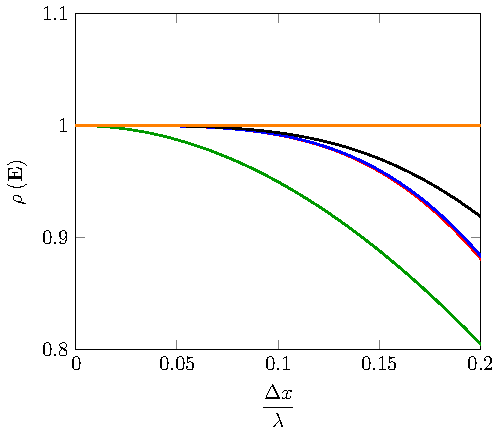
\includegraphics[width=\textwidth]{./chp4/figures/Stabu0khShallz.pdf}\
		\subcaption{$U=0$}
	\end{subfigure}%
	\begin{subfigure}{0.5\textwidth}
		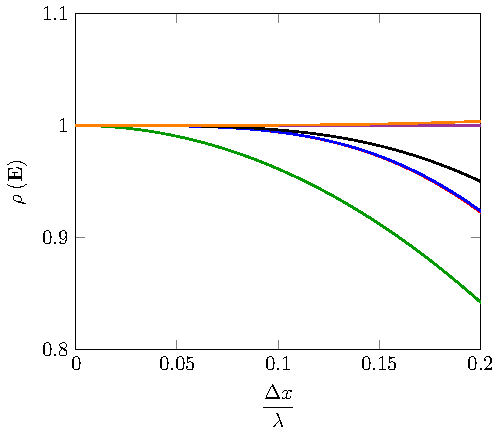
\includegraphics[width=\textwidth]{./chp4/figures/Stabu1khShallz.pdf}
		\subcaption{$U=1$}
	\end{subfigure}
	\caption{Spectral radius of $\matr{E}$ for first-order FDVM ({\color{green!60!black} \solidrule}), second-order FDVM({\color{red} \solidrule}), second-order FEVM ({\color{blue} \solidrule}), third-order FDVM ({\solidrule}), $\mathcal{D}$ ({\color{violet!80!white} \solidrule}) and $\mathcal{W}$ ({\color{orange} \solidrule}). With $H = 1m$ and $k = \frac{\pi}{10}$.}
	\label{fig:StabShall}
\end{figure}




\subsection{Consistency}
For a numerical method to be consistent the error introduced by the method for a single time step must approach zero as the spatial and temporal resolution is increased. To demonstrate the convergence it is enough to demonstrate consistency for the eigenfunctions of the linearised Serre equations, which are the Fourier modes. Therefore, we can demonstrate consistency by investigating the evolution matrix $\matr{E}$. The error introduced for a single time step from $t^n$ to $t^{n+1}$, $\mathcal{T}^n$ is
\begin{equation}
\mathcal{T}^n =  \matr{E}\begin{bmatrix}
\overline{\eta} \\ \overline{G}
\end{bmatrix}^{n}_j -  \begin{bmatrix}
\overline{\eta} \\ \overline{G}
\end{bmatrix}^{n+1}_j.
\label{eqn:consistencyTndef}
\end{equation}
To ensure consistency we must have that $ \lim_{\Delta x,\Delta t \rightarrow 0}\left \| \mathcal{T}^n \right \| = 0 $ for all $n$. Taking the norm of both sides of \eqref{eqn:consistencyTndef} we get

\begin{equation*}
\left \|\mathcal{T}^n \right \| = \left \|  \matr{E}\begin{bmatrix}
\overline{\eta} \\ \overline{G}
\end{bmatrix}^{n}_j - \begin{bmatrix}
\overline{\eta} \\ \overline{G}
\end{bmatrix}^{n+1}_j \right \|.
\label{eqn:consistencyTnnorm1}
\end{equation*}
Making use of \eqref{eqn:fourierfactor} we obtain
\begin{equation*}
\left \|\mathcal{T}^n \right \| = \left \|  \matr{E}\begin{bmatrix}
\overline{\eta} \\ \overline{G}
\end{bmatrix}^{n}_j -  e^{i \omega \Delta t} \begin{bmatrix}
\overline{\eta} \\ \overline{G}
\end{bmatrix}^{n}_j \right \|.
\end{equation*}
Using the matrix norm induced by the vector norm we have that
\begin{equation}
\left \|\mathcal{T}^n \right \|  \le \left \| \matr{E} -  e^{i \omega \Delta t}\matr{I} \right \| \left \| \begin{bmatrix}
\overline{\eta} \\ \overline{G}
\end{bmatrix}^{n}_j\right \|.
\end{equation}
Since $\overline{\eta}^n_j$ and  $\overline{G}^n_j$ are finite and independent of $\Delta x$ and $\Delta t$, if $ \lim_{\Delta x,\Delta t \rightarrow 0}\left \| \matr{E} -  e^{i \omega \Delta t}\matr{I} \right \| = 0 $ then $ \lim_{\Delta x,\Delta t \rightarrow 0}\left \| \mathcal{T}^n \right \| = 0 $ as desired.

We calculated the Taylor series of $\matr{E} -  e^{i \omega_+ \Delta t}\matr{I}$ for all the numerical methods for all flow scenarios; subcritical, critical and supercritical flows. We have reported the lowest order terms of the Taylor series in Tables~\ref{tab:EerrFDVM1}~and~\ref{tab:EerrFDVM1super} for the first-order FDVM, Table~\ref{tab:EerrFDVM2} for the second-order FDVM, Tables~\ref{tab:EerrFDVM3}~and~\ref{tab:EerrFDVM3super} for the third-order FDVM,  Table~\ref{tab:EerrFEVM2} for the second-order FEVM, Table~\ref{tab:EerrD} for $\mathcal{D}$ and Table~\ref{tab:EerrW} for $\mathcal{W}$. To be concise, the temporal and spatial errors for supercritical flow is only reported where it is different from the errors when $-1 \le Fr \le 1$, this only occurred for the spatial errors of the odd-order FDVM. 

We observe for all the methods that the Taylor series of all the elements of $\matr{E} -  e^{i \omega_+ \Delta t}\matr{I}$ have a factor of $\Delta t$. So that for all methods 

\begin{align*}
\left \| \matr{E} -  e^{i \omega_+ \Delta t}\matr{I} \right \| &=  \left \| \Delta t \left(\matr{A}_0 +  \mathcal{O}\left(\Delta t\right)\right)\right \|  \nonumber\\ &= |\Delta t|  \left \| \matr{A}_0 +  \mathcal{O}\left(\Delta t\right)\right \|
 \nonumber\\ &\le  |\Delta t| \left(\left \| \matr{A}_0 \right \| + \left \| \mathcal{O}\left(\Delta t\right)\right \|\right).
\end{align*} 

Choosing a particular vector norm and its induced matrix norm ir is clear from Tables~\ref{tab:EerrFDVM1}-\ref{tab:EerrW} that $\matr{A}_0$ is independent of $\Delta t$ and finite so that as $\Delta t \rightarrow 0$ then $|\Delta t| \left(\left \| \matr{A}_0 \right \| + \left \| \mathcal{O}\left(\Delta t\right)\right \|\right)  \rightarrow 0$  and therefore  $\left \| \matr{E} -  e^{i \omega_+ \Delta t}\matr{I} \right \| \rightarrow 0$. Therefore, for all the numerical methods $ \lim_{\Delta x,\Delta t \rightarrow 0}\left \| \mathcal{T}^n \right \| = 0 $ and so all the numerical methods are consistent for Fourier mode solutions as desired. 

\begin{table}
	\begin{tabular}{l  c c}
	\hline
		Element & \multicolumn{2}{c}{Lowest Order Term of Error}\\
		&  \multicolumn{2}{l}{\rule{0.7\textwidth}{0.4pt}} \\
		& $\Delta x$&$\Delta t$\\
		\hline && \\
		$E_{0,0} -  e^{i \omega_+ \Delta t} $& $ - \frac{1}{2} \sqrt{gH} k^2 \Delta t\Delta x$ & $\dfrac{\sqrt{3gH \beta} + 3U}{\beta} ik \Delta t$ \\ & & \\
		$E_{0,1}$& $ \dfrac{3 + \beta}{4 \beta^2}i k^3\Delta  t\Delta x^2$ &  $ - \frac{3}{\beta} ik\Delta t$ \\ & & \\
		$E_{1,0}$& $ - \frac{1}{2} \sqrt{gH} k^2 \Delta t\Delta x$ &  $ \left(-gH + \dfrac{3U^2}{\beta}\right)ik \Delta t$ \\ & & \\
		$E_{1,1} -  e^{i \omega_+ \Delta t}$& $ - \frac{1}{2} \sqrt{gH} k^2 \Delta t\Delta x$ & $\dfrac{\sqrt{3gH \beta} - 3U}{\beta} ik \Delta t$ \\ 
		\hline
	\end{tabular}
	\caption{Table of the lowest order term of the Taylor series for the elements of $\matr{E} - e^{i \omega_+ \Delta t} \matr{I}$ for the first-order FDVM with $ -1 \le Fr \le 1$ and $\beta = 3 + k^2 H^2$.}
	\label{tab:EerrFDVM1} 
\end{table}

\begin{table}
	\begin{tabular}{l  c  c}
	\hline
		Scheme &\multicolumn{2}{c}{Lowest Order $\Delta x$ Term of Error}\\
		&  \multicolumn{2}{l}{\rule{0.7\textwidth}{0.4pt}} \\
		& $Fr < -1$&$ Fr> 1$\\
		\hline & \\
		$E_{0,0} -  e^{i \omega_+ \Delta t} $& $ \frac{1}{2} k^2 U \Delta t \Delta x$ &  $- \frac{1}{2} k^2 U \Delta t \Delta x$  \\  &  \\
		$E_{0,1}$& $\frac{1}{2}gHk^2 \Delta t \Delta x $ & $\frac{1}{2}gHk^2 \Delta t \Delta x $   \\  &  \\
		$E_{1,1} -  e^{i \omega_+ \Delta t}$& $ \frac{1}{2} k^2 U \Delta t \Delta x$ & $- \frac{1}{2} k^2 U \Delta t \Delta x$   \\ 
	\hline
	\end{tabular}
	\caption{Table of the lowest order term of the Taylor series for the elements of $\matr{E} - e^{i \omega_+ \Delta t} \matr{I}$ for the first-order FDVM which are different than those in Table~\ref{tab:EerrFDVM1}. }
	\label{tab:EerrFDVM1super} 
\end{table}

\begin{table}
	\begin{tabular}{l  c c}
	\hline
		Element & \multicolumn{2}{c}{Lowest Order Term of Error}\\
		&  \multicolumn{2}{l}{\rule{0.7\textwidth}{0.4pt}} \\
		& $\Delta x$&$\Delta t$\\
		\hline && \\
		$E_{0,0} -  e^{i \omega_+ \Delta t} $& $ -\dfrac{i \left(27 + 9H^2k^2 + H^4k^4\right)}{12\beta^2} U k^3 \Delta x^2$ & $\dfrac{\sqrt{3gH \beta} + 3U}{\beta} ik \Delta t$ \\ & & \\
		$E_{0,1}$& $ \dfrac{3 + \beta}{4 \beta^2}i k^3\Delta  t\Delta x^2$ &  $ - \frac{3}{\beta} ik\Delta t$ \\ & & \\
		$E_{1,0}$& $ -\left(gH + \dfrac{3U^2}{\beta} + \dfrac{9U^2}{\beta^2}\right)  \dfrac{k^3}{12}\Delta t\Delta x^2$ &  $ \left(-gH + \dfrac{3U^2}{\beta}\right)ik \Delta t$ \\ & & \\
		$E_{1,1} -  e^{i \omega_+ \Delta t}$& $ \dfrac{-9 + H^2k^2\beta}{\beta^2} \dfrac{k^3}{12} i U \Delta t\Delta x^2$ & $\dfrac{\sqrt{3gH \beta} - 3U}{\beta} ik \Delta t$ \\
		\hline 
	\end{tabular}
	\caption{Table of the lowest order term of the Taylor series for the elements of $\matr{E} - e^{i \omega_+ \Delta t} \matr{I}$ for the second-order FDVM with $ -1 \le Fr \le 1$ and $\beta = 3 + k^2 H^2$.}
	\label{tab:EerrFDVM2} 
\end{table}


\begin{table}
	\begin{tabular}{l  c c}
	\hline
		Element & \multicolumn{2}{c}{Lowest Order Term of Error}\\
		&  \multicolumn{2}{l}{\rule{0.7\textwidth}{0.4pt}} \\
		& $\Delta x$&$\Delta t$\\
		\hline && \\
		$E_{0,0} -  e^{i \omega_+ \Delta t} $& $ - \frac{1}{12} \sqrt{gH} k^4 \Delta t\Delta x^3$ & $\dfrac{\sqrt{3gH \beta} + 3U}{\beta} ik \Delta t$ \\ & & \\
		$E_{0,1}$& $ \dfrac{\sqrt{gH}}{4 \beta}i k^5\Delta  t ^2\Delta x^3$ &  $ - \frac{3}{\beta} ik\Delta t$ \\ & & \\
		$E_{1,0}$& $ - \frac{1}{12} \sqrt{gH} k^4 \Delta t\Delta x^3$ &  $ \left(-gH + \dfrac{3U^2}{\beta}\right)ik \Delta t$ \\ & & \\
		$E_{1,1} -  e^{i \omega_+ \Delta t}$& $ - \frac{1}{12} \sqrt{gH} k^4 \Delta t\Delta x^3$ & $\dfrac{\sqrt{3gH \beta} - 3U}{\beta} ik \Delta t$ \\  \hline
	\end{tabular}
	\caption{Table of the lowest order term of the Taylor series for the elements of $\matr{E} - e^{i \omega_+ \Delta t} \matr{I}$ for the third-order FDVM with $ -1 \le Fr \le 1$ and $\beta = 3 + k^2 H^2$.}
	\label{tab:EerrFDVM3} 
\end{table}

\begin{table}
	\begin{tabular}{l  c  c}
	\hline
		Scheme &\multicolumn{2}{c}{Lowest Order $\Delta x$ Term of Error}\\
		&  \multicolumn{2}{l}{\rule{0.7\textwidth}{0.4pt}} \\
		& $Fr < - 1$&$ Fr >1$\\
		\hline & \\
		$E_{0,0} -  e^{i \omega_+ \Delta t} $& $\frac{1}{12} k^4 U \Delta t \Delta x^3$ &  $ -\frac{1}{12} k^4 U \Delta t \Delta x^3$ \\  &  \\
		$E_{0,1}$& $\dfrac{1}{4 \beta}iUk^5 \Delta t^2 \Delta x^3 $ & $-\dfrac{1}{4 \beta}iUk^5 \Delta t^2 \Delta x^3 $   \\  &  \\
		$E_{1,0}$& $\dfrac{1}{12} gHk^4 \Delta t^2 \Delta x^3 $ & $-\dfrac{1}{12} gHk^4 \Delta t^2 \Delta x^3 $  \\  &  \\
		$E_{1,1} -  e^{i \omega_+ \Delta t}$& $ \frac{1}{12} k^4 U \Delta t \Delta x^3$ & $ -\frac{1}{12} k^4 U \Delta t \Delta x^3$   \\ \hline
	\end{tabular}
	\caption{Table of the lowest order term of the Taylor series for the elements of $\matr{E} - e^{i \omega_+ \Delta t} \matr{I}$ for the third-order FDVM which are different than those in Table~\ref{tab:EerrFDVM1} with  $\beta = 3 + k^2 H^2$. }
	\label{tab:EerrFDVM3super} 
\end{table}

\begin{table}
	\begin{tabular}{l  c c}
	\hline
		Element & \multicolumn{2}{c}{Lowest Order Term of Error}\\
		&  \multicolumn{2}{l}{\rule{0.7\textwidth}{0.4pt}} \\
		& $\Delta x$&$\Delta t$\\
		\hline && \\
		$E_{0,0} -  e^{i \omega_+ \Delta t} $& $ -\dfrac{i \left(54 + 45H^2k^2 + 10H^4k^4\right)}{120\beta^2} U k^3 \Delta t \Delta x^2$ & $\dfrac{\sqrt{3gH \beta} + 3U}{\beta} ik \Delta t$ \\ & & \\
		$E_{0,1}$& $ \dfrac{\beta - 3}{\beta^2} \dfrac{ik^3}{40} \Delta  t\Delta x^2$ &  $ - \frac{3}{\beta} ik\Delta t$ \\ & & \\
		$E_{1,0}$& $ -\left(gH - \dfrac{15U^2}{\beta} + \dfrac{9U^2}{\beta}\right)  \dfrac{k^3}{120}\Delta t\Delta x^2$ &  $ \left(-gH + \dfrac{3U^2}{\beta}\right)ik \Delta t$ \\ & & \\
		$E_{1,1} -  e^{i \omega_+ \Delta t}$& $ \dfrac{126 + 75H^2 k^2 + 10 H^4 k^4}{\beta^2} \dfrac{k^3}{120} i U \Delta t\Delta x^2$ & $\dfrac{\sqrt{3gH \beta} - 3U}{\beta} ik \Delta t$ \\  \hline
	\end{tabular}
	\caption{Table of the lowest order term of the Taylor series for the elements of $\matr{E} - e^{i \omega_+ \Delta t} \matr{I}$ for the second-order FEVM with $ -1 \le Fr \le 1$ and $\beta = 3 + k^2 H^2$.}
	\label{tab:EerrFEVM2} 
\end{table}

\begin{table}
	\begin{tabular}{l  c c}
	\hline
		Element & \multicolumn{2}{c}{Lowest Order Term of Error}\\
		&  \multicolumn{2}{l}{\rule{0.7\textwidth}{0.4pt}} \\
		& $\Delta x$&$\Delta t$\\
		\hline && \\
		$E_{0,0} -  e^{i \omega_+ \Delta t} $&  $\dfrac{ik^3}{3} U \Delta t \Delta x^2$ & $ \sqrt{\dfrac{3gH}{\beta}} 2ik \Delta t $ \\ & & \\
		$E_{0,1}$& $\dfrac{iHk^3}{3} \Delta t \Delta x^2$ &  $-2Hi k \Delta t$ \\ & & \\
		$E_{1,0}$& $ \dfrac{ig \left(3 + \beta\right)}{2\beta^2} k^3\Delta t \Delta x^2$ &  $ -\dfrac{6igk}{\beta} \Delta t$ \\ & & \\
		$E_{1,1} -  e^{i \omega_+ \Delta t}$& $\dfrac{ik^3}{3} U \Delta t \Delta x^2$ & $ \sqrt{\dfrac{3gH}{\beta}} 2ik \Delta t $ \\  \hline
	\end{tabular}
	\caption{Table of the lowest order term of the Taylor series for the elements of $\matr{E} - e^{i \omega \Delta t} \matr{I}$ for $\mathcal{D}$ with $\beta = 3 + k^2 H^2$.}
	\label{tab:EerrD} 
\end{table}

\begin{table}
	\begin{tabular}{l  c c}
	\hline
		Element & \multicolumn{2}{c}{Lowest Order Term of Error}\\
		&  \multicolumn{2}{l}{\rule{0.7\textwidth}{0.4pt}} \\
		& $\Delta x$&$\Delta t$\\
		\hline && \\
		$E_{0,0} -  e^{i \omega_+ \Delta t} $&  $\dfrac{ik^3}{6} U \Delta t \Delta x^2$ & $ \sqrt{\dfrac{3gH}{\beta}} ik \Delta t $ \\ & & \\
		$E_{0,1}$& $\dfrac{iHk^3}{6} \Delta t \Delta x^2$ &  $-Hi k \Delta t$ \\ & & \\
		$E_{1,0}$& $ \dfrac{ig \left(3 + \beta\right)}{2\beta^2} k^3\Delta t \Delta x^2$ &  $ -\dfrac{6igk}{\beta} \Delta t$ \\ & & \\
		$E_{1,1} -  e^{i \omega_+ \Delta t}$& $\dfrac{ik^3}{3} U \Delta t \Delta x^2$ & $ \sqrt{\dfrac{3gH}{\beta}} 2ik \Delta t $ \\  \hline
	\end{tabular}
	\caption{Table of the lowest order term of the Taylor series for the elements of $\matr{E} - e^{i \omega_+ \Delta t} \matr{I}$ for $\mathcal{W}$ with $\beta = 3 + k^2 H^2$.}
	\label{tab:EerrW} 
\end{table}




\section{Dispersion Analysis}
To study the dispersion of the numerical methods $\omega$ for the numerical methods must be calculated. Making use of \eqref{eqn:fourierfactor} in \eqref{eqn:evolutionmatrix} we get 
\begin{equation}
e^{i \omega \Delta t}\begin{bmatrix}
\overline{\eta} \\ \overline{G}
\end{bmatrix}^{n}_j =  \matr{E}\begin{bmatrix}
\overline{\eta} \\ \overline{G}
\end{bmatrix}^{n}_j.
\label{eqn:dispanalomeganum1}
\end{equation}
Assuming that $\matr{E}$ has an eigenvalue decomposition $\matr{E} = \matr{P}^{-1} \matr{\Lambda} \matr{P}$ and substituting it into \eqref{eqn:dispanalomeganum1} we get
\begin{equation}
e^{i \omega \Delta t}\begin{bmatrix}
\overline{\eta} \\ \overline{G}
\end{bmatrix}^{n}_j =  \matr{P}^{-1} \matr{\Lambda} \matr{P}\begin{bmatrix}
\overline{\eta} \\ \overline{G}
\end{bmatrix}^{n}_j.
\label{eqn:dispanalomeganum2}
\end{equation}
Left multiplying \eqref{eqn:dispanalomeganum2} by $\matr{P}$ we obtain
\begin{equation}
e^{i \omega \Delta t} \matr{P}\begin{bmatrix}
\overline{\eta} \\ \overline{G}
\end{bmatrix}^{n}_j =   \matr{\Lambda} \matr{P}\begin{bmatrix}
\overline{\eta} \\ \overline{G}
\end{bmatrix}^{n}_j.
\label{eqn:dispanalomeganum3}
\end{equation}
Since $\Lambda$ is a diagonal matrix we must have that $e^{i \omega_+ \Delta t} = \lambda_+$ and $e^{i \omega_- \Delta t} = \lambda_-$ where $\lambda_\pm$ are the eigenvalues of $\matr{E}$ and $\omega_\pm$ are the positive and negative branches of the dispersion relation. Therefore, the dispersion relation of a numerical method is
\begin{equation}
\widetilde{\omega}_\pm = \frac{1}{i \Delta t} \log\left[ \lambda_\pm\right].
\end{equation}
By comparing $\widetilde{\omega}_\pm$ with the analytic $\omega_\pm$ given by the linearised Serre equations \eqref{eqn:DispersionRelation} we can determine the error in the dispersion relation for the numerical method. The real part of $\widetilde{\omega}_\pm$ determines the speed of a wave, while the imaginary part determines the change in amplitude. For $\omega_\pm$ the imaginary part is zero and so the amplitude of waves of the linearised Serre equations are constant in time. We only present the results for the positive branch of the dispersion relation as the results for the negative and positive branches are very similar. 

The relative error in the dispersion relation was plotted against $\Delta x / \lambda$ for representative values of $H$, $U$ and $k$.  We used $g = 9.81m/s^2$ and chose $\Delta t = 0.5 / \left(U + \sqrt{gH}\right) \Delta x$ to satisfy the CFL condition \eqref{eqn:CFLcond}.

In Figures~\ref{fig:Dispu0Shall}~and~\ref{fig:Dispu1Shall} we present the plots for $kH = \pi / 10$ so that the water is shallow as $\sigma = 1 / 20$ and therefore, the Serre equations are appropriate. We present the real and imaginary errors separately as they account for different physical phenomenon and also present the total relative error as a measure of the overall difference of behaviour between waves in the numerical method and the waves of the linearised Serre equations.

From Figures~\ref{fig:Dispu0Shall}~and~\ref{fig:Dispu1Shall} we can see that all methods approximate the dispersion relation of the Serre equations well with the approximation improving as $\Delta x \rightarrow 0$, as expected.

For the real part of the dispersion error the FEVM and the FDVM outperform the two finite difference methods and therefore will better approximate the speed of waves of the linearised Serre equations.  However, for the dilation of waves the roles are reversed with the two finite difference methods either dilating the waves very little ($\mathcal{W}$ for $U>0$) or not at all. When taking both effects into account with the complete error we see that the first-order FDVM has the largest dispersion error followed by $\mathcal{W}$, $\mathcal{D}$, the second-order FEVM, the second-order FDVM and finally the third-order FDVM has the lowest dispersion error. So that the size of the total dispersion error is mainly determined by the order of accuracy of the numerical scheme. These results justify choosing the hybrid methods over these finite difference methods for the Serre equations. 

Figures~\ref{fig:Dispu0Shall}~and~\ref{fig:Dispu1Shall} furthermore demonstrate that the second-order FDVM is superior to the FEVM not just for the complete dispersion error, but its real and imaginary parts individually as well. Therefore, the second-order FDVM will do a better job in accurately modelling the speed and amplitude of waves than the second-order FEVM. Interestingly, for the two finite difference methods and the first-order FDVM there seems to be some trade-off between predicting the speed or amplitude of the waves very well. 

We observed similar results across a wide array of $k$, $H$ and $U$ values. However, as $kH$ is increased the distinction between the second-order FDVM and the second-order FEVM becomes less pronounced. This can be seen in Figure~\ref{fig:Dispu0Fill} where $kH = 2.5$ and $\sigma = 5/4 \pi > 1/20$ so that the water is no longer shallow.

These $kH$ values are the same as those by \citet{Filippini-etal-2016-381}, and our results are similar for the real part of the dispersion error. Our FDVM and the FEVM compare favourably with the methods described and analysed by \citet{Filippini-etal-2016-381}. Furthermore, we extended their work by allowing for non-zero values of $U$, combining the spatial and temporal approximations and examining the imaginary and complete error in the dispersion relation. 

Figure~\ref{fig:Dispu1Fill} demonstrates that the results of the real part of the dispersion error  is slightly different if we allow for non-zero values of $U$. In particular the non-zero value of $U$ changes the real part of the dispersion error for the first-order FDVM, most significantly when $kH = 2.5$. Therefore, for some methods allowing for non-zero values of $U$ can have a significant impact on the conclusions drawn from the dispersion analysis. Furthermore, taking the imaginary part of the dispersion error into account is important as $\omega$ determines not only the speed of waves but also their amplitude. In particular it is possible that a method like the first-order FDVM performs very well for the real part of the dispersion error and poorly for the imaginary part, leading to false conclusions about the accuracy of the method.


\begin{figure}
	\centering
	\begin{subfigure}{0.5\textwidth}
		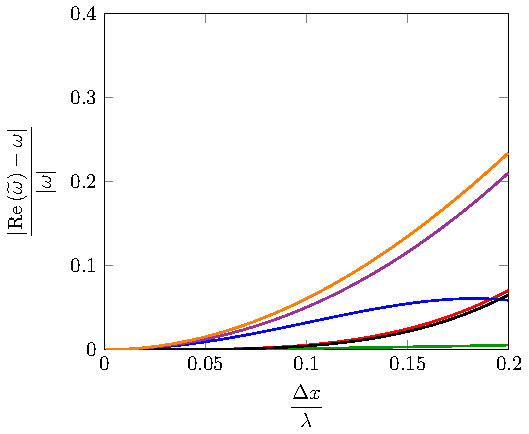
\includegraphics[width=\textwidth]{./chp4/figures/Dispu0khShallRez.pdf}
		\subcaption{Real Part}
	\end{subfigure}%
	\begin{subfigure}{0.5\textwidth}
		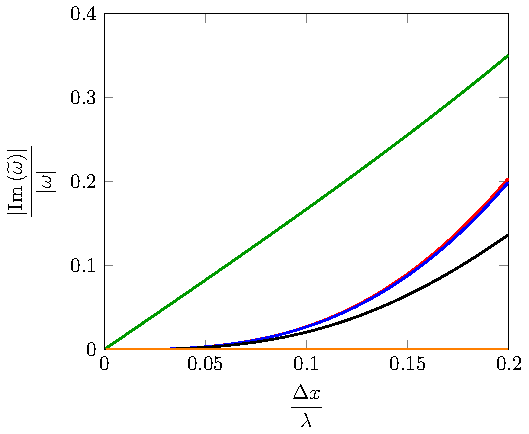
\includegraphics[width=\textwidth]{./chp4/figures/Dispu0khShallImz.pdf}
		\subcaption{Imaginary Part}
	\end{subfigure}
	\par\bigskip
	\begin{subfigure}{0.5\textwidth}
		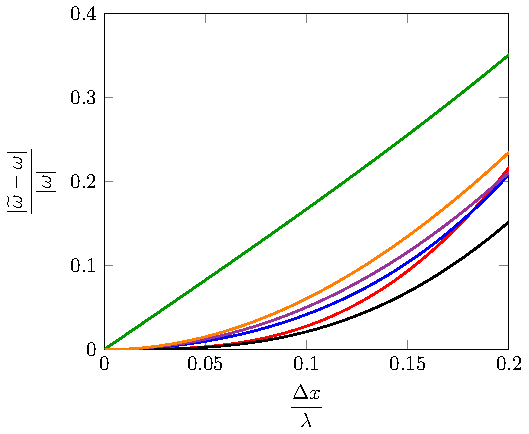
\includegraphics[width=\textwidth]{./chp4/figures/Dispu0khShallz.pdf}
		\subcaption{Real and Imaginary Parts}
	\end{subfigure}
	\caption{Relative dispersion error for first-order FDVM ({\color{green!60!black} \solidrule}), second-order FDVM({\color{red} \solidrule}), second-order FEVM ({\color{blue} \solidrule}), third-order FDVM ({\solidrule}), $\mathcal{D}$ ({\color{violet!80!white} \solidrule}) and $\mathcal{W}$ ({\color{orange} \solidrule}). With $H = 1m$, $k = \frac{\pi}{10}$ and $U = 0 m/s$.}
	\label{fig:Dispu0Shall}
\end{figure}

\begin{figure}
	\centering
	\begin{subfigure}{0.5\textwidth}
		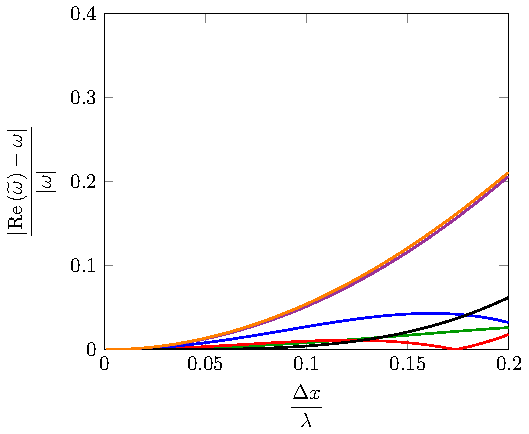
\includegraphics[width=\textwidth]{./chp4/figures/Dispu1khShallRez.pdf}
		\subcaption{Real part}
	\end{subfigure}%
	\begin{subfigure}{0.5\textwidth}
		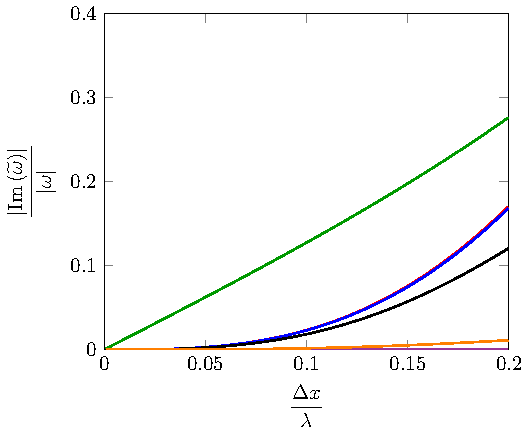
\includegraphics[width=\textwidth]{./chp4/figures/Dispu1khShallImz.pdf}
		\subcaption{Imaginary part}
	\end{subfigure}
	\par\bigskip
	\begin{subfigure}{0.5\textwidth}
		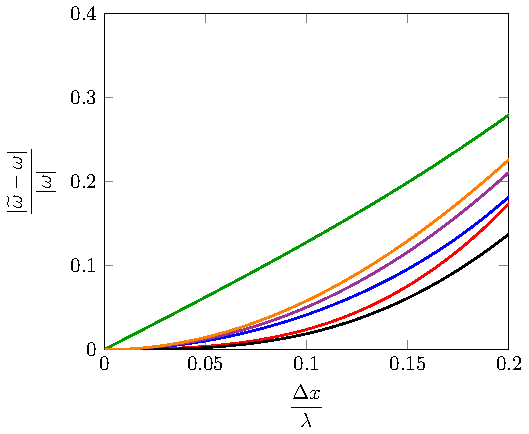
\includegraphics[width=\textwidth]{./chp4/figures/Dispu1khShallz.pdf}
		\subcaption{Real and Imaginary Parts}
	\end{subfigure}
	\caption{Relative dispersion error for first-order FDVM ({\color{green!60!black} \solidrule}), second-order FDVM({\color{red} \solidrule}), second-order FEVM ({\color{blue} \solidrule}), third-order FDVM ({\solidrule}), $\mathcal{D}$ ({\color{violet!80!white} \solidrule}) and $\mathcal{W}$ ({\color{orange} \solidrule}). With $H = 1m$, $k = \frac{\pi}{10}$ and $U = 1 m/s$.}
	\label{fig:Dispu1Shall}
\end{figure}

\begin{figure}
	\centering
	\begin{subfigure}{0.5\textwidth}
		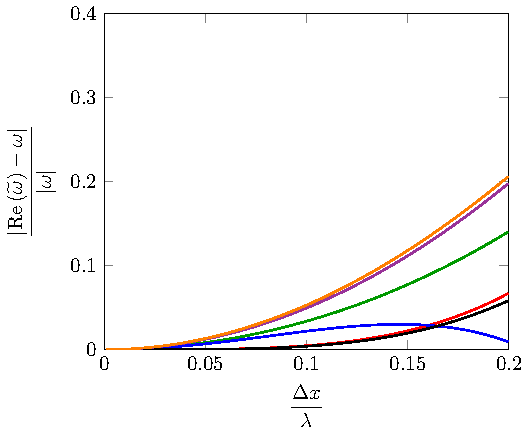
\includegraphics[width=\textwidth]{./chp4/figures/Dispu0khFillRez.pdf}
		\subcaption{Real part}
	\end{subfigure}%
	\begin{subfigure}{0.5\textwidth}
		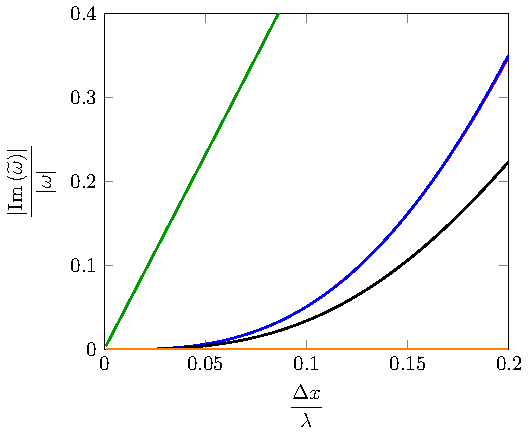
\includegraphics[width=\textwidth]{./chp4/figures/Dispu0khFillImz.pdf}
		\subcaption{Imaginary part}
	\end{subfigure}
	\par\bigskip
	\begin{subfigure}{0.5\textwidth}
		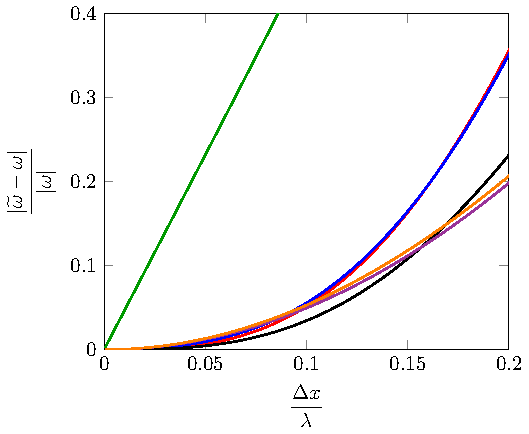
\includegraphics[width=\textwidth]{./chp4/figures/Dispu0khFillz.pdf}
		\subcaption{Real and Imaginary Parts}
	\end{subfigure}
	\caption{Relative dispersion error for first-order FDVM ({\color{green!60!black} \solidrule}), second-order FDVM({\color{red} \solidrule}), second-order FEVM ({\color{blue} \solidrule}), third-order FDVM ({\solidrule}), $\mathcal{D}$ ({\color{violet!80!white} \solidrule}) and $\mathcal{W}$ ({\color{orange} \solidrule}). With $H = 1m$, $k = 2.5$ and $U = 0m/s$.}
	\label{fig:Dispu0Fill}
\end{figure}

\begin{figure}
	\centering
	\begin{subfigure}{0.5\textwidth}
		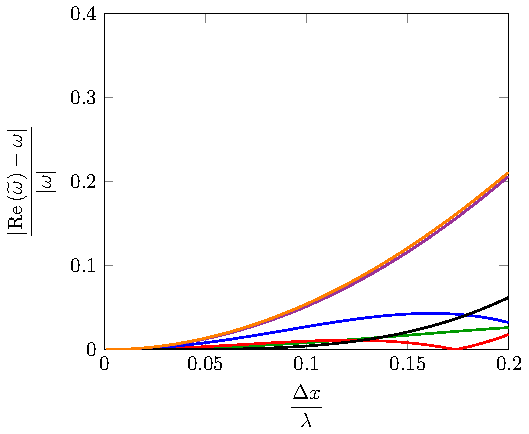
\includegraphics[width=\textwidth]{./chp4/figures/Dispu1khFillRez.pdf}
		\subcaption{Real part}
	\end{subfigure}%
	\begin{subfigure}{0.5\textwidth}
		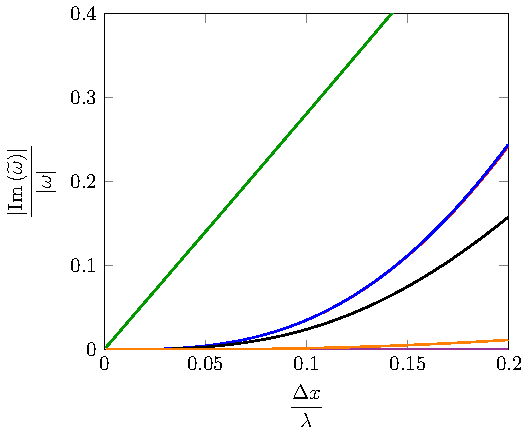
\includegraphics[width=\textwidth]{./chp4/figures/Dispu1khFillImz.pdf}
		\subcaption{Imaginary part}
	\end{subfigure}
	\par\bigskip
	\begin{subfigure}{0.5\textwidth}
		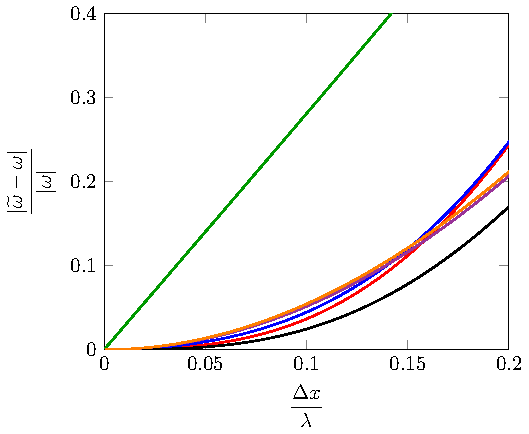
\includegraphics[width=\textwidth]{./chp4/figures/Dispu1khFillz.pdf}
		\subcaption{Real and Imaginary Parts}
	\end{subfigure}
	\caption{Relative dispersion error for first-order FDVM ({\color{green!60!black} \solidrule}), second-order FDVM({\color{red} \solidrule}), second-order FEVM ({\color{blue} \solidrule}), third-order FDVM ({\solidrule}), $\mathcal{D}$ ({\color{violet!80!white} \solidrule}) and $\mathcal{W}$ ({\color{orange} \solidrule}). With $H = 1m$, $k = 2.5$ and $U = 1m/s$.}
	\label{fig:Dispu1Fill}
\end{figure}


The Taylor series expansion of $\widetilde{\omega}$ was also derived for all the numerical methods. We have compiled the lowest order terms of the Taylor series for $\widetilde{\omega}_+-\omega_+$ in Table \ref{tab:Wfactor} when $ -1 \le Fr \le 1$ for the FDVM and FEVM. In Table \ref{tab:Wfactor} it is clear that these schemes estimated $\omega$ with the expected order of accuracy in both space and time.

We also present the lowest order terms of the Taylor series for $\widetilde{\omega}_+~-~\omega_+$ for both $ Fr < -1$ and $ Fr > 1$ in Table~\ref{tab:Wspatfactor}. We only present the errors that are different from those reported in Table~\ref{tab:Wfactor}, this was only the case for the spatial error of the odd-order numerical methods. We can see that for all the flow scenarios that our FDVM and the FEVM have the correct order of accuracy when approximating $\omega_+$. 

Finally we present the lowest order terms of the Taylor series for $\widetilde{\omega}_+~-~\omega_+$ for the finite difference methods in Table~\ref{tab:WFDspatfactor}. These methods do not change depending on the value of the physical quantities. The two finite difference methods both have the correct order of accuracy in space and time.  

Because all methods were demonstrated to have the expected order of accuracy in approximating $\omega_+$ this implies that for small $\Delta x$ values the order of accuracy will be the primary driver of the dispersion error.

	\begin{table}
		\begin{tabular}{l  c  c}
		\hline
			Scheme & \multicolumn{2}{c}{Lowest Order Term of Error}\\
			&  \multicolumn{2}{l}{\rule{0.7\textwidth}{0.4pt}} \\
			& $\Delta x$&$\Delta t$\\
			\hline && \\
			$\text{FDVM}_1$& $-\left(2 \sqrt{gH} - \sqrt{\dfrac{3U}{\beta }}\right)  \dfrac{ik^2}{4} \Delta x$ & $\dfrac{i \omega_+^2}{2} \Delta t$ \\ & & \\
			$\text{FDVM}_2$& $\dfrac{2\beta U -3 \sqrt{3 gH \beta}}{\beta^2}  \dfrac{k^3}{24}\Delta x ^2$ & $- \dfrac{\omega^3_+}{6 }  \Delta t^2$ \\ & & \\
			$\text{FEVM}_2$& $\left(U   + \dfrac{\left(42 + 15 k^2H^2\right) \sqrt{3gH \beta}}{20\beta^2}  \right) \dfrac{k^3}{12 } \Delta x^2$ &  $- \dfrac{\omega^3_+}{6 }  \Delta t^2$  \\ & & \\
			$\text{FDVM}_3$& $-\left({2\sqrt{gH} - \sqrt{3\beta}U }\right) \dfrac{ik^4}{24} \Delta x^3$ & $-\dfrac{i\omega^4_+}{24 } \Delta t^3$ \\ \hline
		\end{tabular}
		\caption{Table showing lowest order error term for approximating $\omega_+$ for all FDVM and the FEVM. With $  -1 \le Fr \le 1$ and $\beta = 3 + H^2 k^2 $. }
		\label{tab:Wfactor} 
	\end{table}

	\begin{table}
		\begin{tabular}{l  c  c}
		\hline
			Scheme &\multicolumn{2}{c}{Lowest Order $\Delta x$ Term of Error}\\
				&  \multicolumn{2}{l}{\rule{0.7\textwidth}{0.4pt}} \\
				& $Fr < - 1$&$ Fr >1$\\
			\hline & \\
			$\text{FDVM}_1$& $-\left(2U + \sqrt{\dfrac{3gH}{\beta}}\right)  \dfrac{ik^2}{4} \Delta x$ &  $\left(2U + \sqrt{\dfrac{3gH}{\beta}}\right)  \dfrac{ik^2}{4} \Delta x$  \\  &  \\
			$\text{FDVM}_3$& $-\left(2U + \sqrt{\dfrac{3gH}{\beta}} \right) \dfrac{ik^4}{24} \Delta x^3$ & $\left(2U + \sqrt{\dfrac{3gH}{\beta}} \right) \dfrac{ik^4}{24} \Delta x^3$   \\  &  \\
			\hline
		\end{tabular}
		\caption{Table showing the lowest order spatial error term for approximating $\omega_+$ for all FDVM and the FEVM for supercritical Froude numbers where different from Table \ref{tab:Wfactor}. With $\beta = 3 + H^2 k^2 $. }
		\label{tab:Wspatfactor} 
	\end{table}
	
		\begin{table}
		\begin{tabular}{l  c  c}
		\hline
			Scheme & \multicolumn{2}{c}{Lowest Order Term of Error}\\
			&  \multicolumn{2}{l}{\rule{0.7\textwidth}{0.4pt}} \\
			& $\Delta x$&$\Delta t$\\
			\hline && \\
			$\mathcal{D}$& $- \left(U + \dfrac{\left( 4 + H^2k^2\right)\sqrt{3gH\beta}}{4 \beta^2}\right)\dfrac{k^3}{3 }\Delta x^2$  &$ -\dfrac{\omega_+^3}{3}\Delta t^2$ \\ & & \\
			$\mathcal{W}$& $\left(U + \dfrac{\left( 4 + H^2k^2\right)\sqrt{3gH\beta}}{4 \beta^2}\right)\dfrac{k^3}{3 }\Delta x^2$  &$ \Bigg( \beta U^2\left[9\sqrt{3gH \beta} + 4 \beta U\right]  $  \\ & & $+ 3gH^2\left[\sqrt{3gH \beta} + 6 \beta U\right] \Bigg) \dfrac{k^3}{18 \beta^2}\Delta t^2$ \\\hline
		\end{tabular}
			\caption{Table showing lowest order error term for approximating $\omega_+$ for $\mathcal{D}$ and $\mathcal{W}$. }
			\label{tab:WFDspatfactor} 
		\end{table}

 %W x orig :  \dfrac{gH\left( 4 + H^2k^2\right)}{2 \beta \sqrt{3gH\beta}}
